\section{Data Storage}
  \subsection{Session}
    Session that determining which user is currently posting request is stored in redis which is a light key-value pair database.
    Though only one value can be stored with one key, its high performance makes it's the best to store sessions data.

    The sessions is stored automaticly without any design, for a third party package will handle all of this.

  \subsection{Item}
    Item mainly is the only things that we need to store other than user's information which needed for all apps.
    An item will be mapped into a FetcherContext object in program, and it will be stored into database simply with all attributes
    by key-value pair.

    \begin{figure}[H]
      \centering
      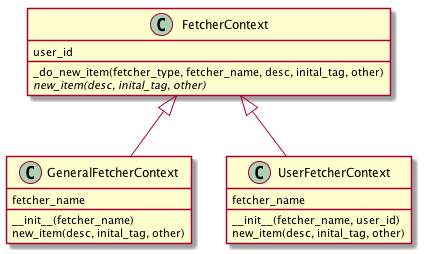
\includegraphics[width=0.6\textwidth]{img/fetcherContext.png}
      \caption{FetcherContext\label{fig:fetcherContext}}
    \end{figure}
